%!TEX root = handout.tex

\setcounter{equation}{0}

%%%%%%%%%%%%%%%%%%%%%%%%%%%%%%%%%%%%%%%%%%%%%%%%%%%%%%%%%%%%%%%%%%%%%%%%%%%%%%%%
\section{Getting started}

\subsection{Data conversion}
\label{Data_Conversion}

Each MS instrument vendor has one or more formats for storing the acquired data. Converting these data into an open format (preferably mzML) is the very first step when you want to work with open-source mass spectrometry software. A freely available conversion tool is ProteoWizard. The OpenMS installation package for Windows automatically installs ProteoWizard, so you do not need to download and install it separately.

Please note that due to restrictions from the instrument vendors, file format conversion for most formats is only possible on Windows systems, so exporting from the acquisition PC connected to the instrument is usually the most convenient option.
All files used in this tutorial have already been converted to mzML by us, so you do not need to do it yourself.

%%%%%%%%%%%%%%%%%%%%%%%%%%%%%%%%%%%%%%%%%%%%%%%%%%%%%%%%%%%%%%%%%%%%%%%%%%%%%%%%

\subsection{Data visualization using \OPENMSTOOL{TOPPView}}
\label{Data_Visualization}

Visualizing the data is the first step in quality control, an essential tool in understanding the data, and of course an essential step in pipeline development.
OpenMS provides a convenient viewer for some of the data: \OPENMSTOOL{TOPPView}.

We will guide you through some of the basic features of \OPENMSTOOL{TOPPView}. Please familiarize yourself with the key controls and visualization methods.
We will make use of these later throughout the tutorial. Let's start with a first look at one of the files of our tutorial data set:

\begin{itemize}
\item Start \OPENMSTOOL{TOPPView} (see Start-Menu or Applications on MacOS)
\item Go to \menu{File > Open File}, navigate to the directory where you copied the contents of the USB stick to,
      and select
      \directory{ OpenMS / small / velos005614.mzML}
      . This file contains a reduced LC-MS map (only a selected RT and m/z range
      was extracted using the TOPP tool FileFilter) of a label-free measurement of the human platelet proteome recorded on an Orbitrap velos.
      The other two mzML files contain technical replicates of this experiment.
\item Play around.
\item Three action modes are supported, one for scrolling, one for zooming and one for measuring:
    \begin{itemize}
    \item Scroll mode
        \begin{itemize}
        \item It is activated by default, though each loaded spectra file is displayed zoomed out first, so you do not need to scroll.
        \item When zommed in, to scroll the spectra map, click-drag on the current view.
        \item Arrow keys can be used to scroll the view as well.
        \end{itemize}
    \item Zoom mode
        \begin{itemize}
        \item All previous zoom levels are stored in a zoom history. The zoom history can be traversed using
              \keys[,]{\ctrl,+} or \keys[,]{\ctrl,-} or the mouse wheel (scroll up and down).
        \item Zooming into the data: either mark an area in the current view with your mouse while holding the left mouse
              button plus the \keys{\ctrl} key to zoom to this area
              or use your mouse wheel to traverse the zoom history.
        \item If you have reached the end of the history and keep on pressing \keys[,]{\ctrl,+} or
        			scroll up, the current area will be enlarged by a factor of $1.25$
        \item Pressing the Backspace key resets the zoom and zoom history.
        \end{itemize}
    \item Measure mode
        \begin{itemize}
        \item It is activated using the \keys{\shift} key.
        \item Press the left mouse button down while a peak is selected and drag the mouse to
        			another peak to measure the distance between peaks.
        \item This mode is implemented in the 1D and 2D mode only.
        \end{itemize}
    \end{itemize}
\item Right click on your 2D map and select \menu{Switch to 3D view} and examine your
			data in 3D mode
\item Go back to the 2D view. In 2D mode, visualize your data in different normalization modes, use linear, percentage and log-view (icons on the upper left tool bar).
\note{On \textit{Apple OS X}, due to a bug in one of the external libraries used by OpenMS, you will see a small window of the 3D mode when switching to 2D. Close the 3D tab in order to get rid of it.}
\item In \OPENMSTOOL{TOPPView} you can also execute TOPP tools. Go to
			\menu{Tools > Apply tool (whole layer)} and choose a TOPP tool (e.g., FileInfo) and
			inspect the results.
\end{itemize}

%%%%%%%%%%%%%%%%%%%%%%%%%%%%%%%%%%%%%%%%%%%%%%%%%%%%%%%%%%%%%%%%%%%%%%%%%%%%%%%%

\subsection{Introduction to KNIME / OpenMS}
\label{KNIME_Intro}

Using OpenMS in combination with KNIME you can create, edit, open, save, and run workflows
combining TOPP tools with the powerful data analysis capabilities of KNIME. Workflows can
be created conveniently in a graphical user interface. The parameters of all involved
tools can be edited within the application and are also saved as part of the workflow.
Furthermore, KNIME interactively performs validity checks during the workflow editing
process, in order to make it more difficult to create an invalid workflow.

Throughout most of the parts of this tutorial you will use KNIME to create and
execute workflows. This first step is to make yourself familiar with KNIME.

\subsubsection{Install OpenMS using KNIME}

Before we can start with the tutorial we need to install all the required extension for KNIME.
First we will install the OpenMS plugin, providing all the OpenMS nodes.
Afterwards we will install some additional plugins that we will use in the more advanced part of this tutorial.

\begin{enumerate}
\item Open KNIME.
\item Click on \menu{Help > Install New Software...}
\item \label{it:add_site} In the now open dialog choose \menu{Add...} (in the upper right corner of the dialog) to define a new update site. In the opening dialog enter the following details. \\
\textit{Name:} \texttt{Trunk Community Contributions} \\
\textit{Location:} \texttt{http://tech.knime.org/update/community-contributions/trunk/}
\item \label{it:select_site} After pressing \keys{OK} KNIME will show you all the contents of the added Update Site, containing also the OpenMS nodes.
%\todo{First install File Handling Nodes?}
\item Select the OpenMS nodes in the category "KNIME Community Contributions - Bioinformatics \& NGS" and click \keys{Next}.
\item Follow the instructions and after a restart of KNIME the OpenMS nodes will be available under “Community Nodes”.
\end{enumerate}

\note{
For this tutorial we use a pre-release version of OpenMS 1.12.
While not being a full release, it was nevertheless intensively tested to ensure its functionality for this tutorial.
For regular use we recommend using the latest stable OpenMS release.
To install the latest stable release skip Steps \ref{it:add_site} and \ref{it:select_site} and instead choose the update site \menu{Trusted Community Contributions}.
Please note that some of the workflows shown here require OpenMS 1.12 and therefore will not work with OpenMS 1.11.1 downloaded from the stable update site.
}

For the rest of the tutorial we will also need some more plugins, that can be installed similar to the OpenMS nodes.

\begin{enumerate}
\item Again, click on \menu{Help > Install New Software...}
\item From the \menu{Work with:} drop down list select the \menu{KNIME Analytics Platform Update Site}
\item Now select the following plugins from the \textit{KNIME \& Extensions} category
    \begin{itemize}
    \item KNIME Base Chemistry Types \& Nodes
    \item KNIME Chemistry Add-Ons
    \item KNIME File Handling Nodes
    \item KNIME Interactive R Statistics Integration
    \item KNIME Math Expression (JEP)
    \item KNIME Report Designer
    \item KNIME SVG Support
    \item KNIME XLS Support
    \item KNIME XML-Processing
    \end{itemize}
\item And the following plugin from the \textit{Marvin Chemistry Extensions (donated by Infocom \& Chemaxon)} category
    \begin{itemize}
    \item ChemAxon/Infocom Marvin Extensions Feature
    \end{itemize}
\item Click \keys{Next} and follow the instructions.
\end{enumerate}

\subsubsection{KNIME Concepts}

A \textbf{workflow} is a sequence of steps applied to a single or multiple input data sets to process and analyse this data.
In KNIME such workflows are implemented graphically by combining so-called \textbf{nodes}.

A node represents a single analysis step in a workflow.
Nodes have input and output ports where the data goes into to the node or the results are provided for other nodes after processing, respectively.
KNIME distinguishes between different port types, representing different types of data.
The most common representation in KNIME are tables (similar to an excel sheet).
Those ports are marked with a small triangle.
For OpenMS we use a different port type, so called file ports, representing complete files.
Those ports are marked by a small grey box.
Dark grey boxes represent mandatory inputs and light grey boxes optional inputs.

Nodes can have three different states, indicated by the small traffic light below the node.

\begin{itemize}
\item
Inactive, failed, and not yet fully configured nodes are marked red.
\item
Configured but not yet executed nodes are marked yellow.
\item
Successfully executed nodes are marked green.
\end{itemize}

If the node execution failed the node will switch to the red state.

Most nodes will be configured as soon as all input ports are connected.
For some nodes additional parameters have to be provided that cannot be either guessed from the data or filled with sensible defaults.
In this case, of if you want to customise the default configuration, you can open the configuration dialog of a node with a double-click on the node.
For OpenMS you will see a configuration dialog like the one shown in \cref{fig:knime_configure}.
\note{OpenMS distinguishes between normal parameters and advanced parameters.
Advanced parameters are by default hidden from the users since they should only rarely be customised.
In case you want to have a look at the parameters or need to customise them in one of the tutorials you can show them by clicking on the checkbox  \menu{Show advanced parameter} in the lower part of the dialog.}
The dialog shows the individual parameters, their current value and type, and, in the lower part of the dialog, the documentation for the currently selected parameter.

\begin{figure}
\centering
\includegraphics[width=0.5\textwidth]{graphics/knime_setup/knime_configure_dialog}
\caption{Node configuration dialog of an OpenMS node.}
\label{fig:knime_configure}
\end{figure}

\subsubsection{Overview of the graphical user interface}

\begin{figure}
\includegraphics[width=\textwidth]{graphics/knime_setup/knime_workbench_marked}
\caption{The KNIME workbench.}
\label{fig:knime_workbench}
\end{figure}

The graphical user interface (GUI) of KNIME consists of different components or so called panels that are shown in \cref{fig:knime_workbench}.
We will shortly introduce the individual panels and their purpose below.

\begin{description}
\item[Workflow Editor]
The workflow editor is the central part of the KNIME GUI.
Here you assemble the workflow by adding nodes from the Node Repository via "drag \& drop".
Nodes can be connected by clicking on the output port of one node and releasing the mouse at the desired input port of the next node.

\item[Workflow Explorer]
Shows a list of available workflows (also called workflow projects).
You can open a workflow by double clicking it.
A new workflow can be created with a right-click in the Workflow Explorer followed by selecting \menu{New KNIME Workflow...}.

\item[Node Repository]
Shows all nodes that are available in your KNIME installation.
Every plugin you install will provide new nodes that can be found here.
The OpenMS nodes can be found in \menu{Community Nodes > OpenMS}.
Nodes for managing files (e.g., Input Files or Output Folders) can be found in \menu{Community Nodes > GenericKnimeNodes}.
You can search the node repository by typing the node name into the small text box in the upper part of the node repository.

\item[Outline]
The Outline panel contains a small overview of the complete workflow. While of limited use when working on a small workflow, this feature is very helpful as soon as the workflows get bigger.

\item[Console]
In the console panel warning and error messages are shown.
This panel will provide helpful information if one of the nodes failed or shows an warnings sign.

\item[Node Description]
As soon as a node is selected, the Node Description window will show the documentation of the node including documentation for all its parameters.
For OpenMS nodes you will also find a link to the tool page in the online documentation.

\end{description}

\subsubsection{Creating workflows}
\label{sec:create_workflows}

Workflows can easily be created by a right click in the Workflow Explorer followed by clicking on \menu{New KNIME Workflow...}.

\subsubsection{Sharing workflows}
\label{sec:sharing_workflows}

To be able to share a workflow with others KNIME supports the import and export of complete workflows.
To export a workflow select it in the Workflow Explorer and select \menu{File > Export KNIME Workflow...}.
KNIME will export workflows as a zip file containing all the information on nodes, their connections, and their configuration.
Those zip files can again be imported by selecting \menu{File > Import KNIME Workflow...}.

\note{For your convenience we added all workflows discussed in this tutorial to the \directory{Workflows} folder.
If you want to check your own workflow by comparing it to the solution or got stuck, simply import the full workflow from the corresponding zip file.}

\subsubsection{Duplicating workflows}
\label{sec:duplicate-wf}

During the tutorial a lot of the workflows will be created based on the workflow from a previous task.
To keep the intermediate workflows we suggest you create copies of your workflows so you can see the progress.
To create a copy of your workflow follow the following steps

\begin{itemize}
\item
Right click on the workflow you want to create a copy of in the Workflow Explorer and select \menu{Copy}.
\item
Right click again somewhere on the workflow explorer and select \menu{Paste}.
\item
This will create a workflow with same name as the one you copied with a (2) appended.
\item
To distinguish them later on you can easily rename the workflows in the Workflow Explorer by right clicking on the workflow and selecting \menu{Rename}. \note{To rename a workflow it has to be closed.}
\end{itemize}

\subsubsection{A minimal workflow}
\label{Minimal_Workflow}

Let us now start with the creation of our very first, very simple workflow.
As a first step, we will gather some basic information about the data set before starting the
actual development of a data analysis workflow.

\begin{itemize}
\item
Create a new workflow.
\item Add an \KNIMENODE{Input File} node and an \KNIMENODE{Output Folder} node (to be found in \menu{Community Nodes > GenericKnimeNodes > IO} and a \KNIMENODE{FileInfo} node (to be found in the category \menu{Community Nodes > OpenMS > File Handling}) to the workflow.
\item Connect the \KNIMENODE{Input File} node to the \KNIMENODE{FileInfo} node, and the first output port of the \KNIMENODE{FileInfo} node to the \KNIMENODE{Output Folder} node.
\note{In case you are unsure about which node port to use, hovering the cursor over the port in question will display the port name and what kind of input it expects.}
The complete workflow is shown in \cref{fig:knime_minimal}.
FileInfo can produce two different kinds of output files.
\item All nodes are still marked red, since we are missing an actual input file.
Double-click the Input File node and select \menu{Browse}.
In the file system browser select \directory{OpenMS / tiny / velos005614.mzML} and click \menu{Open}.
Afterwards close the dialog by clicking \menu{Ok}.
\note{Make sure to use the ``tiny'' version this time, not ``small'', for the sake of faster workflow execution.}
\item The \KNIMENODE{Input File} node and the \KNIMENODE{FileInfo} node should now have switched to yellow, but the \KNIMENODE{Output Folder} node is still red.
Double-click on the \KNIMENODE{Output Folder} node and click on \menu{Browse} to select an output directory for the generated data.
\item Great! Your first workflow is now ready to be run. Press \keys{\shift + F7} to execute the complete workflow.
You can also right click on any node of your workflow and select \menu{Execute} from the context menu.
\item The traffic lights tell you about the current status of all nodes in your workflow.
Currently running tools show either a progress in percent or a moving blue bar, nodes waiting for data show the small word ``queued'', and successfully executed ones become green.
If something goes wrong (e.g., a tool crashes), the light will become red.
\item In order to inspect the results, you can just right-click the \KNIMENODE{Output Folder} node and select \menu{View: Open the output folder}.
You can then open the text file and inspect its contents.
You will find some basic information of the data contained in the mzML file, e.g., the total number of spectra and peaks, the RT and m/z range, and how many MS1 and MS2 spectra the file contains.
\end{itemize}

\begin{figure}
\centering
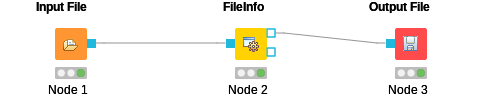
\includegraphics[width=0.59\textwidth]{graphics/knime_setup/Minimal_FileInfo}
\caption{A minimal workflow calling FileInfo on a single file.}
\label{fig:knime_minimal}
\end{figure}

Now consider you would like to gather this information for more then one file.
We will now modify the workflow to compute the same information on three different files and then write the output files to a folder.

\begin{itemize}
\item
We start from the previous workflow.
\item
First we need to replace our single input file with multiple files.
Therefore we add the \KNIMENODE{Input Files} node from the category \menu{Community Nodes > GenericKnimeNodes > IO}.
\item
To select the files we double-click on the \KNIMENODE{Input Files} node and click on \menu{Add}.
In the filesystem browser we select all three files from the directory \directory{OpenMS / tiny / }.
And close the dialog with \menu{Ok}.
\item
We now add two more nodes: the \KNIMENODE{ZipLoopStart} and the \KNIMENODE{ZipLoopEnd} node from the category \menu{Community Nodes > GenericKnimeNodes > Flow}.
\item
Afterwards we connect the \KNIMENODE{Input Files} node to the first port of the \KNIMENODE{ZipLoopStart} node, the first port of the \KNIMENODE{ZipLoopStart} node to the \KNIMENODE{FileInfo} node, the first output port of the \KNIMENODE{FileInfo} node to the first input port of the \KNIMENODE{ZipLoopEnd} node, and the first output port of the \KNIMENODE{ZipLoopEnd} node to the \KNIMENODE{Output Folder} node (, not \KNIMENODE{Output File}).
The complete workflow is shown in \cref{fig:knime_minimal_loop}
\item
The workflow is already complete.
Simply execute the workflow and inspect the output as before.
\end{itemize}

\begin{figure}
\centering
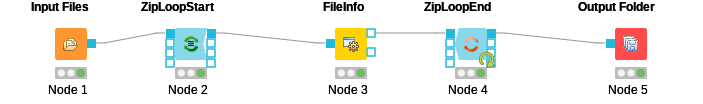
\includegraphics[width=\textwidth]{graphics/knime_setup/Minimal_FileInfoLoop}
\caption{A minimal workflow calling FileInfo on multiple files in a loop.}
\label{fig:knime_minimal_loop}
\end{figure}
